\subsubsection{Caso d'uso UC8.1.3.4: Wizard creazione domanda di collegamento}
\label{UC8.1.3.4}
\begin{figure}[h]
	\centering
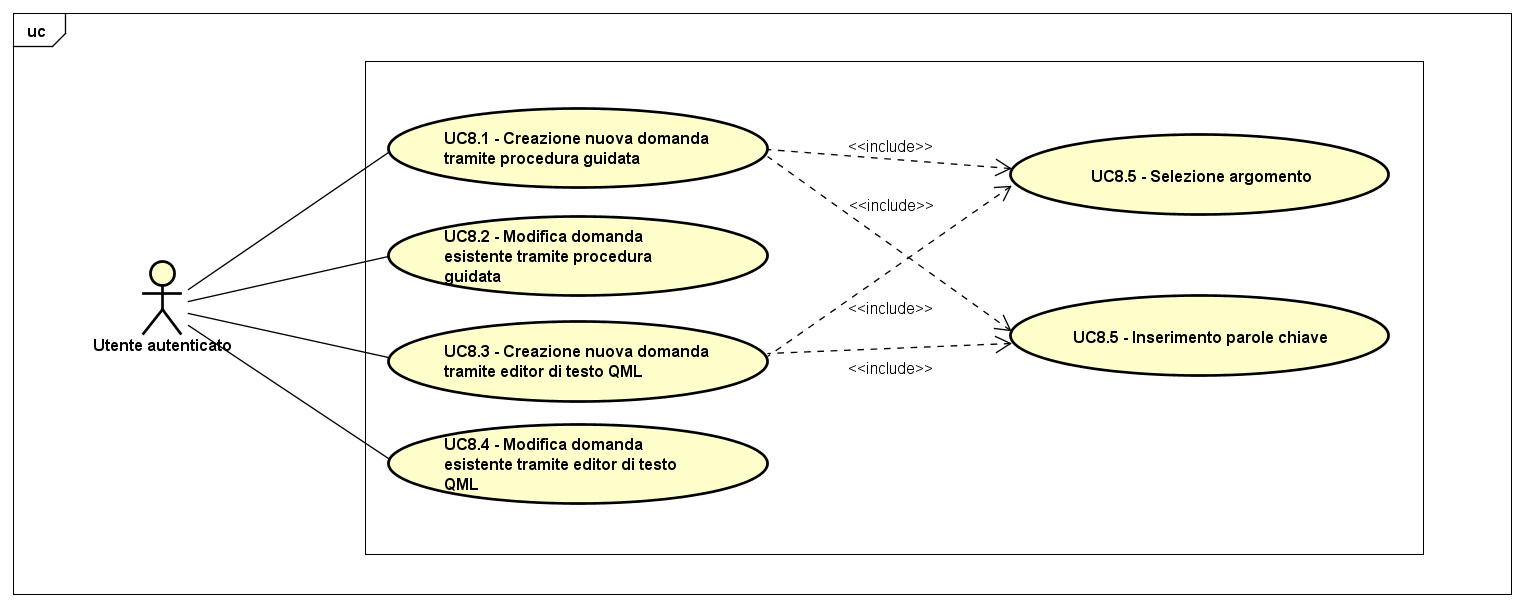
\includegraphics[scale=0.5,keepaspectratio]{UML/UC8.png}
	\caption{Caso d'uso UC8.1.3.4: Wizard creazione domanda di collegamento}
\end{figure}
\FloatBarrier
\begin{itemize}
	\item \textbf{Attori}: \uau, \uaupro;
	\item \textbf{Descrizione}: l'attore utilizza la procedura guidata per la creazione di una domanda di tipo collegamento. 
	\item \textbf{Precondizione}: l'attore ha scelto l'opzione "Wizard creazione domanda di collegamento" nelle scelte possibili nel caso d'uso UC8.1.3;
	\item \textbf{Postcondizione}: l'attore ha completato tutte i campi necessari per la creazione di una domanda di tipo collegamento;
	\item \textbf{Scenario principale}: 
		\begin{enumerate}
			\item L'attore inserisce una coppia di vocaboli (UC8.1.3.4.1)
			\item L'attore può eliminare una coppia di vocaboli appena inserita (UC8.1.3.4.2)
		\end{enumerate}
\end{itemize}







\subsubsection{Caso d'uso UC8.1.3.4: k}
\label{UC8.1.3.4.}
\begin{figure}[h]
	\centering
	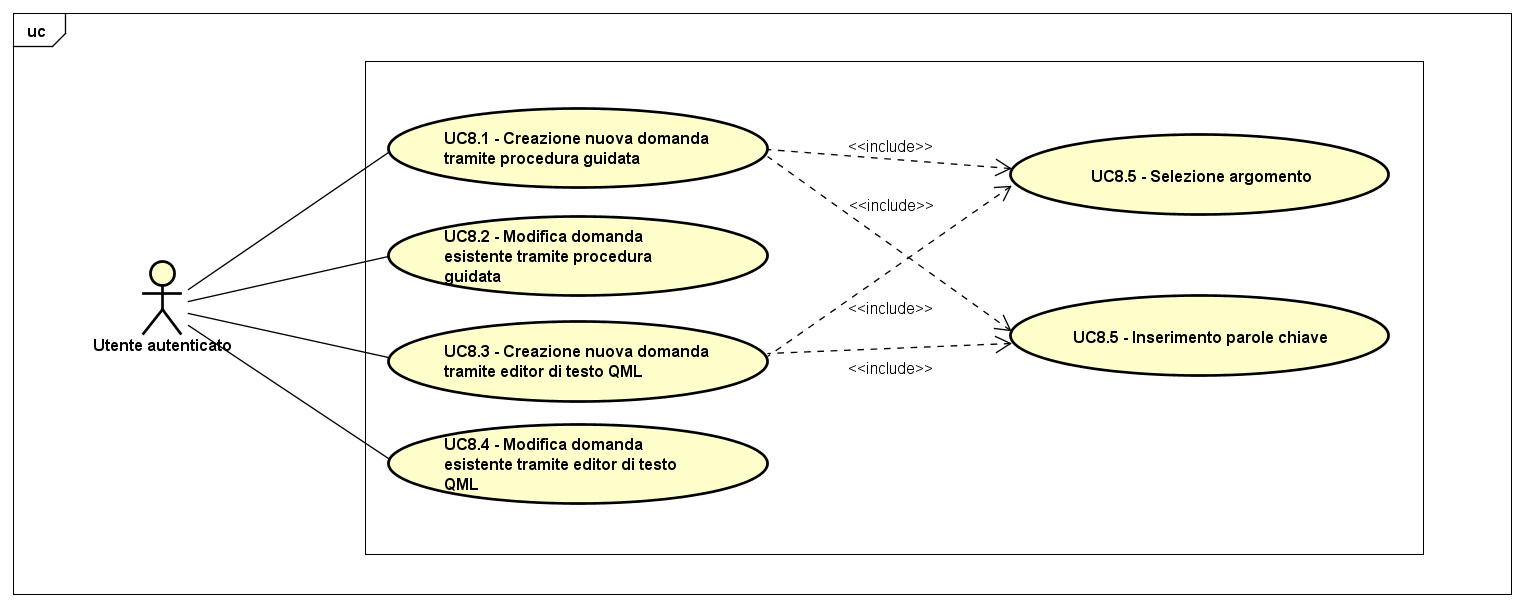
\includegraphics[scale=0.5,keepaspectratio]{UML/UC8.png}
	\caption{Caso d'uso UC8.1.3.4: k}
\end{figure}
\FloatBarrier
\begin{itemize}
	\item \textbf{Attori}: 
	\item \textbf{Descrizione}:
	\item \textbf{Precondizione}: 
	\item \textbf{Postcondizione}: 
	\item \textbf{Scenario principale}: 
	\begin{enumerate}
		\item
	\end{enumerate}
	\item \textbf{Inclusioni}: 
	\item \textbf{Estensioni}: 
	\item \textbf{Scenari alternativi}: 
\end{itemize}